% Options for packages loaded elsewhere
\PassOptionsToPackage{unicode}{hyperref}
\PassOptionsToPackage{hyphens}{url}
%
\documentclass[
]{article}
\usepackage{amsmath,amssymb}
\usepackage{iftex}
\ifPDFTeX
  \usepackage[T1]{fontenc}
  \usepackage[utf8]{inputenc}
  \usepackage{textcomp} % provide euro and other symbols
\else % if luatex or xetex
  \usepackage{unicode-math} % this also loads fontspec
  \defaultfontfeatures{Scale=MatchLowercase}
  \defaultfontfeatures[\rmfamily]{Ligatures=TeX,Scale=1}
\fi
\usepackage{lmodern}
\ifPDFTeX\else
  % xetex/luatex font selection
\fi
% Use upquote if available, for straight quotes in verbatim environments
\IfFileExists{upquote.sty}{\usepackage{upquote}}{}
\IfFileExists{microtype.sty}{% use microtype if available
  \usepackage[]{microtype}
  \UseMicrotypeSet[protrusion]{basicmath} % disable protrusion for tt fonts
}{}
\makeatletter
\@ifundefined{KOMAClassName}{% if non-KOMA class
  \IfFileExists{parskip.sty}{%
    \usepackage{parskip}
  }{% else
    \setlength{\parindent}{0pt}
    \setlength{\parskip}{6pt plus 2pt minus 1pt}}
}{% if KOMA class
  \KOMAoptions{parskip=half}}
\makeatother
\usepackage{xcolor}
\usepackage[left=1cm,right=1cm,top=1cm,bottom=1cm]{geometry}
\usepackage{graphicx}
\makeatletter
\def\maxwidth{\ifdim\Gin@nat@width>\linewidth\linewidth\else\Gin@nat@width\fi}
\def\maxheight{\ifdim\Gin@nat@height>\textheight\textheight\else\Gin@nat@height\fi}
\makeatother
% Scale images if necessary, so that they will not overflow the page
% margins by default, and it is still possible to overwrite the defaults
% using explicit options in \includegraphics[width, height, ...]{}
\setkeys{Gin}{width=\maxwidth,height=\maxheight,keepaspectratio}
% Set default figure placement to htbp
\makeatletter
\def\fps@figure{htbp}
\makeatother
\setlength{\emergencystretch}{3em} % prevent overfull lines
\providecommand{\tightlist}{%
  \setlength{\itemsep}{0pt}\setlength{\parskip}{0pt}}
\setcounter{secnumdepth}{-\maxdimen} % remove section numbering
\pagenumbering{gobble} \usepackage{float} \floatplacement{figure}{H}
\ifLuaTeX
  \usepackage{selnolig}  % disable illegal ligatures
\fi
\usepackage{bookmark}
\IfFileExists{xurl.sty}{\usepackage{xurl}}{} % add URL line breaks if available
\urlstyle{same}
\hypersetup{
  pdftitle={Paleorecords reveal biological mechanisms critical for reliable species range shift projections amid rapid climate change},
  pdfauthor={V. Van der Meersch et al.},
  hidelinks,
  pdfcreator={LaTeX via pandoc}}

\title{Paleorecords reveal biological mechanisms critical for reliable
species range shift projections amid rapid climate change}
\usepackage{etoolbox}
\makeatletter
\providecommand{\subtitle}[1]{% add subtitle to \maketitle
  \apptocmd{\@title}{\par {\large #1 \par}}{}{}
}
\makeatother
\subtitle{Figures for manuscript and extended data}
\author{V. Van der Meersch et al.}
\date{}

\begin{document}
\maketitle

\section{Main}\label{main}

\begin{figure}
\centering
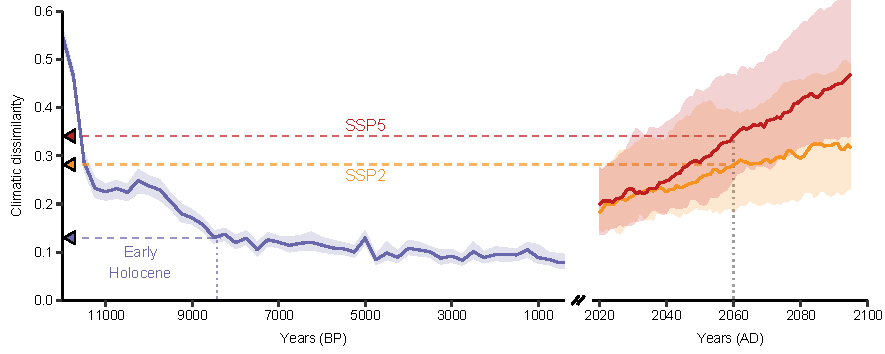
\includegraphics{/home/victor/projects/past_robustness/manuscript/figs/files/climatic_dissimilarity-1.pdf}
\caption{Evolution of climatic dissimilarity under past (12k-500 yr BP)
and future (2005-2100) climate changes, relative to 1901-2000\}.}
\end{figure}

\newpage

\begin{figure}
\centering
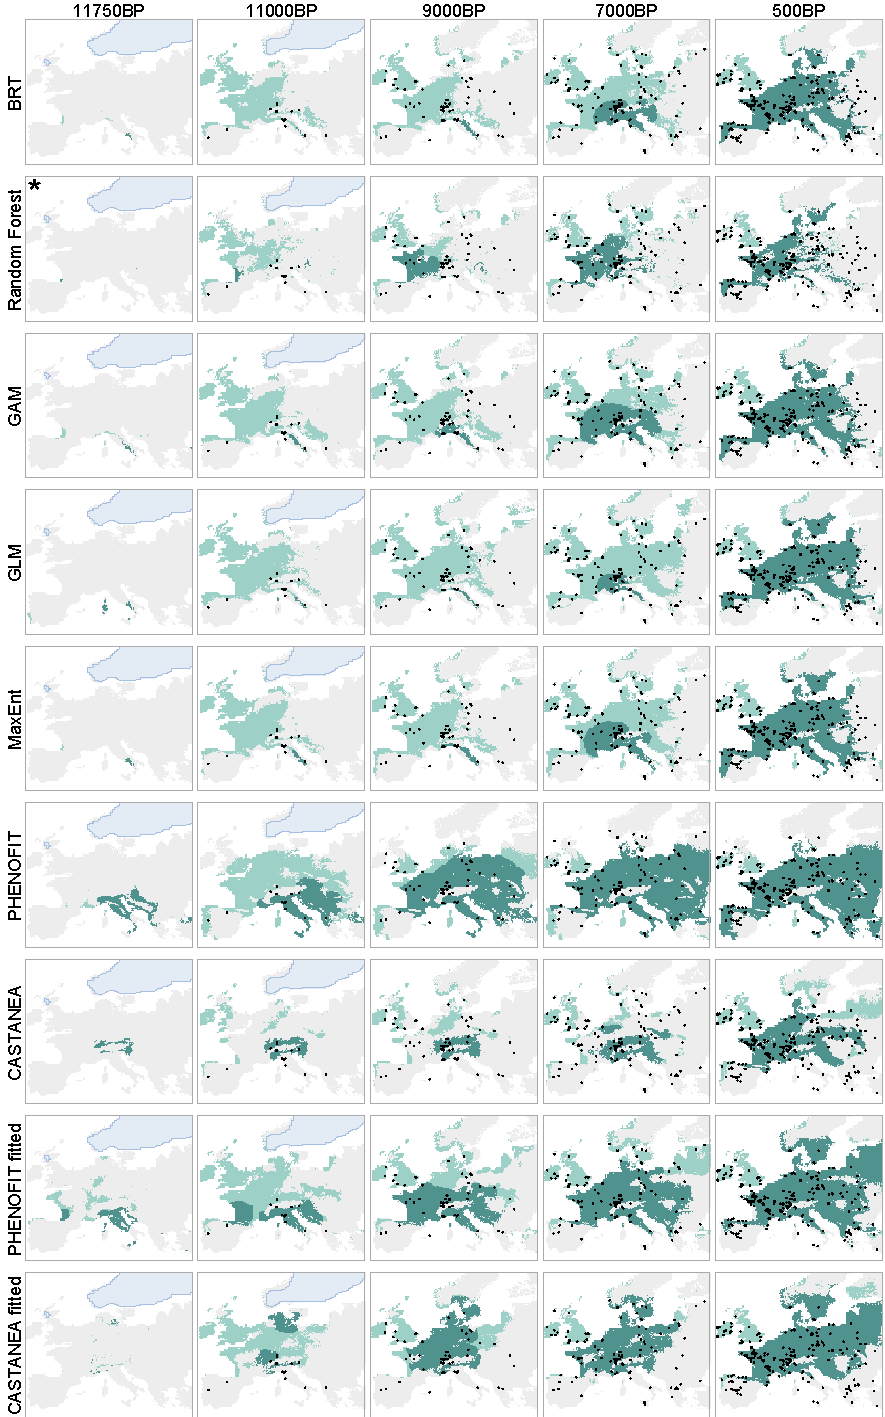
\includegraphics{/home/victor/projects/past_robustness/manuscript/figs/files/quercus_deciduous_simulations-1.pdf}
\caption{Example of paleosimulations obtained with the eight models used
in this study for deciduous oaks.}
\end{figure}

\newpage

\begin{figure}
\centering
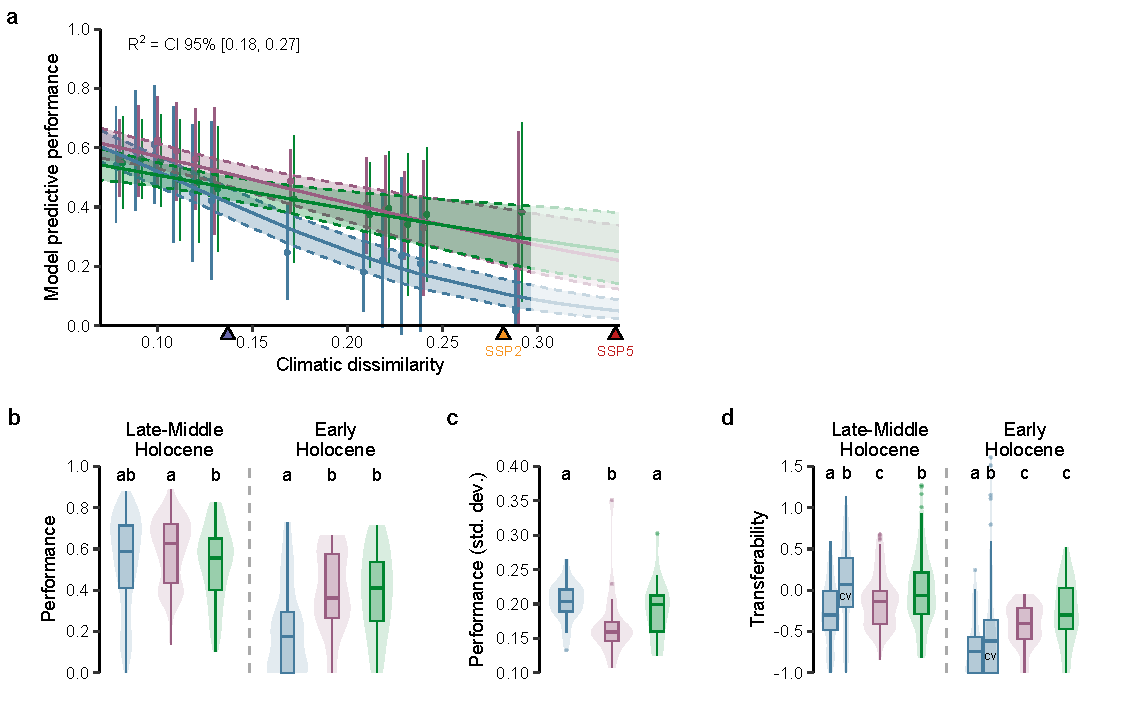
\includegraphics{/home/victor/projects/past_robustness/manuscript/figs/files/past_performance-1.pdf}
\caption{Performance of correlative models, fitted process-based models
(inverse calibration using occurrence data) and expert process-based
models (classical calibration) against Holocene paleoecogical evidence
(fossil pollen) for 4 tree genera.}
\end{figure}

\newpage

\section{Supplementary data}\label{supplementary-data}

\renewcommand{\thefigure}{S\arabic{figure}}
\setcounter{figure}{0}

\begin{figure}
\centering
\includegraphics{/home/victor/projects/past_robustness/manuscript/figs/files/figS1_climate_overview-1.pdf}
\caption{Chronology of past climate across the Late Pleistocene and the
Holocene.}
\end{figure}

\begin{figure}
\centering
\includegraphics{/home/victor/projects/past_robustness/manuscript/figs/files/figS2_climatic_dissimilarity_novelty-1.pdf}
\caption{Evoltion of climatic dissimilarity/novelty in past and future.}
\end{figure}

\begin{figure}
\centering
\includegraphics{/home/victor/projects/past_robustness/manuscript/figs/files/figs4_fagus_simulations-1.pdf}
\caption{Example of paleosimulations obtained with the eight models used
in this study for beeches.}
\end{figure}

\begin{figure}
\centering
\includegraphics{/home/victor/projects/past_robustness/manuscript/figs/files/figS5_abies_simulations-1.pdf}
\caption{Example of paleosimulations obtained with the eight models used
in this study for firs.}
\end{figure}

\begin{figure}
\centering
\includegraphics{/home/victor/projects/past_robustness/manuscript/figs/files/figS6_quercusevergreen_simulations-1.pdf}
\caption{Example of paleosimulations obtained with the eight models used
in this study for evergreen oaks.}
\end{figure}

\begin{figure}
\centering
\includegraphics{/home/victor/projects/past_robustness/manuscript/figs/files/figS7_migration_process_stochasticity-1.pdf}
\caption{Illustration of migration process and evaluation of the impact
of migration process stochasticity.}
\end{figure}

\section{Additionnal figures after
review}\label{additionnal-figures-after-review}

\begin{figure}
\centering
\includegraphics{/home/victor/projects/past_robustness/manuscript/figs/files/figS10_SDMclass-1.pdf}
\caption{Sensitivity, difference across models.}
\end{figure}

\begin{figure}
\centering
\includegraphics{/home/victor/projects/past_robustness/manuscript/figs/files/figSX_refugia-1.pdf}
\caption{Refugia.}
\end{figure}

\section{Modified figure after second round of
review}\label{modified-figure-after-second-round-of-review}

\includegraphics{/home/victor/projects/past_robustness/manuscript/figs/files/different_initial_refugia-1.pdf}

\end{document}
